\section{IPMA}

\subsection{International Project Management Association}
\begin{frame}[allowframebreaks]{International Project Management Association}
	IPMA \foreign{International Project Management Association}
	\begin{itemize}
		\item Asociación Internacional dedicada al desarrollo y promoción de la \textbf{dirección de proyectos}.
		\item Organizada como una federación internacional de más de 55 asociaciones nacionales de dirección y gestión de proyectos.
		\item Su actividad principal es la \textbf{certificación} de las competencias en dirección de proyectos.
		\item ICB \foreign{(IPMA Competence Baseline)}
		\begin{itemize}
				\item Marco desarrollado para las habilidades en dirección de proyectos, que sirve de base para el programa de certificación en \textbf{cuatro niveles}.
		\end{itemize}
		\item La certificación abarca competencias técnicas, contextuales y del comportamiento, y ha de renovarse cada cierto tiempo.
	\end{itemize}
	
	\framebreak
	
	Un poco de historia
	
	\begin{itemize}
		\item El origen de la IPMA se remonta a 1964 cuando un grupo internacional de directores de proyectos se reunió para discutir los beneficios del método de la ruta crítica.
		\item En 1965 este grupo de debate fundó en Suiza una asociación, la actual IPMA, bajo el nombre de IMSA \foreign{(International Management Systems Association)}.
		\item El primer congreso internacional tuvo lugar en 1967 en Viena, con participantes de 30 países diferentes.
	\end{itemize}
	
	\framebreak
	
	Niveles de certificación que establece IPMA en dirección de proyectos:
	
	\begin{enumerate}
		\item IPMA Nivel A \emph{(Certified Projects Director)}
		\item IPMA Nivel B \emph{(Certified Senior Project Manager)}
		\item IPMA Nivel C \emph{(Certified Project Manager)}
		\item IPMA Nivel D \emph{(Certified Project Management Associate)}
	\end{enumerate}
	
	\framebreak
	
	\begin{block}{IPMA Nivel A \emph{(Certified Projects Director)}}
		\begin{itemize}
			\item Competencias: Será capaz de gestionar carteras o programas.
			\item Requisitos: Para obtenerlo se debe tener como mínimo cinco años de experiencia en dirección de carteras, dirección de programas o dirección de multiproyectos.
		\end{itemize}
	\end{block}
	
		\begin{block}{IPMA Nivel B \emph{(Certified Senior Project Manager)}}
			\begin{itemize}
				\item Competencias: Será capaz de dirigir proyectos complejos.
				\item Requisitos: Para obtenerlo se debe tener como mínimo cinco años de experiencia en dirección de proyectos.
			\end{itemize}
		\end{block}
	
	\framebreak
	
	\begin{block}{IPMA Nivel C \emph{(Certified Project Manager)}}
		\begin{itemize}
			\item Competencias: Será capaz de dirigir proyectos de complejidad limitada o de gestionar un subproyecto de un proyecto complejo en todos los elementos de competencia de la dirección de proyectos.
			\item Requisitos: Para obtenerlo se debe tener como mínimo tres años de experiencia en dirección de proyectos.
		\end{itemize}
	\end{block}
	
	\begin{block}{IPMA Nivel D \emph{(Certified Project Management Associate)}}
		\begin{itemize}
			\item Competencias: Tendrá conocimientos de dirección de proyectos en todos los elementos de competencia.
			\item Requisitos: No es obligatoria ninguna experiencia previa para obtenerlo.
		\end{itemize}
	\end{block}
	
	\framebreak
	
	Beneficios de los programas de certificación:
	
	\begin{itemize}
		\item Para el personal de dirección de proyectos: obtener un certificado con reconocimiento internacional que dé fe de su competencia en la dirección.
		\item Para los proveedores de servicios de dirección de proyectos: una demostración de la competencia profesional de sus empleados.
		\item Para los clientes: Mayor certeza de que recibirán los servicios más avanzados de un director de proyectos.
	\end{itemize}
\end{frame}

\subsection{AEIPRO (IPMA en España)}

\begin{frame}[allowframebreaks]{AEIPRO (IPMA en España)}
	AEIPRO \foreign{Asociación Española de Ingeniería de Proyectos}
	\begin{itemize}
		\item Asociación sin ánimo de lucro que tiene por objetivo el desarrollo del campo de la Dirección e Ingeniería de Proyectos.
		\item Nace en 1992 y desde el año 1999 es la asociación española representante de IPMA \foreign{(International Project Management Association)}.
	\end{itemize}
	
	\framebreak
	
	Para conseguir el proceso de certificación en España de IPMA(AEIPRO) se han de seguir los siguientes pasos:
	
	\begin{enumerate}
		\item El aspirante a conseguir la certificación en dirección de proyectos debe contactar con la secretaría del OCDP (aeipro@dpi.upv.es) indicando su interés por participar en alguna de las convocatorias previstas y el nivel solicitado.
		\item La secretaría remitirá la aceptación preliminar y pedirá al aspirante que envíe la "Solicitud de Evaluación" correspondiente al nivel solicitado, en la que se incluyen y explican los modelos a cumplimentar por el aspirante.
		\item El aspirante justifica el abono de la tasa y firma la solicitud devolviéndola a la secretaría, así como los impresos de currículum vitae (formato incluido en la solicitud) y autoevaluación debidamente cumplimentados, y los impresos de justificación de experiencia en su caso.
		\framebreak
		\item Una vez estudiada la documentación, la secretaría devuelve:
		\begin{itemize}
			\item Aceptación o denegación como candidato para iniciar el proceso de certificación.
			\item El comprobante de pago de la devolución (en caso de no aceptación).
			\item Notificación para la asistencia a la prueba.
		\end{itemize}
		\item El candidato realiza la prueba.
		\item La secretaría informa de los resultados directamente al candidato y de los pasos siguientes que procedan.
		\item La secretaría actualiza los registros de certificados para que los recién incorporados figuren en el Libro de Certificados de IPMA del año en curso. Y, finalmente, se entrega el diploma acreditativo al ahora ya recién certificado.
		
		\framebreak
		
		\begin{center}
			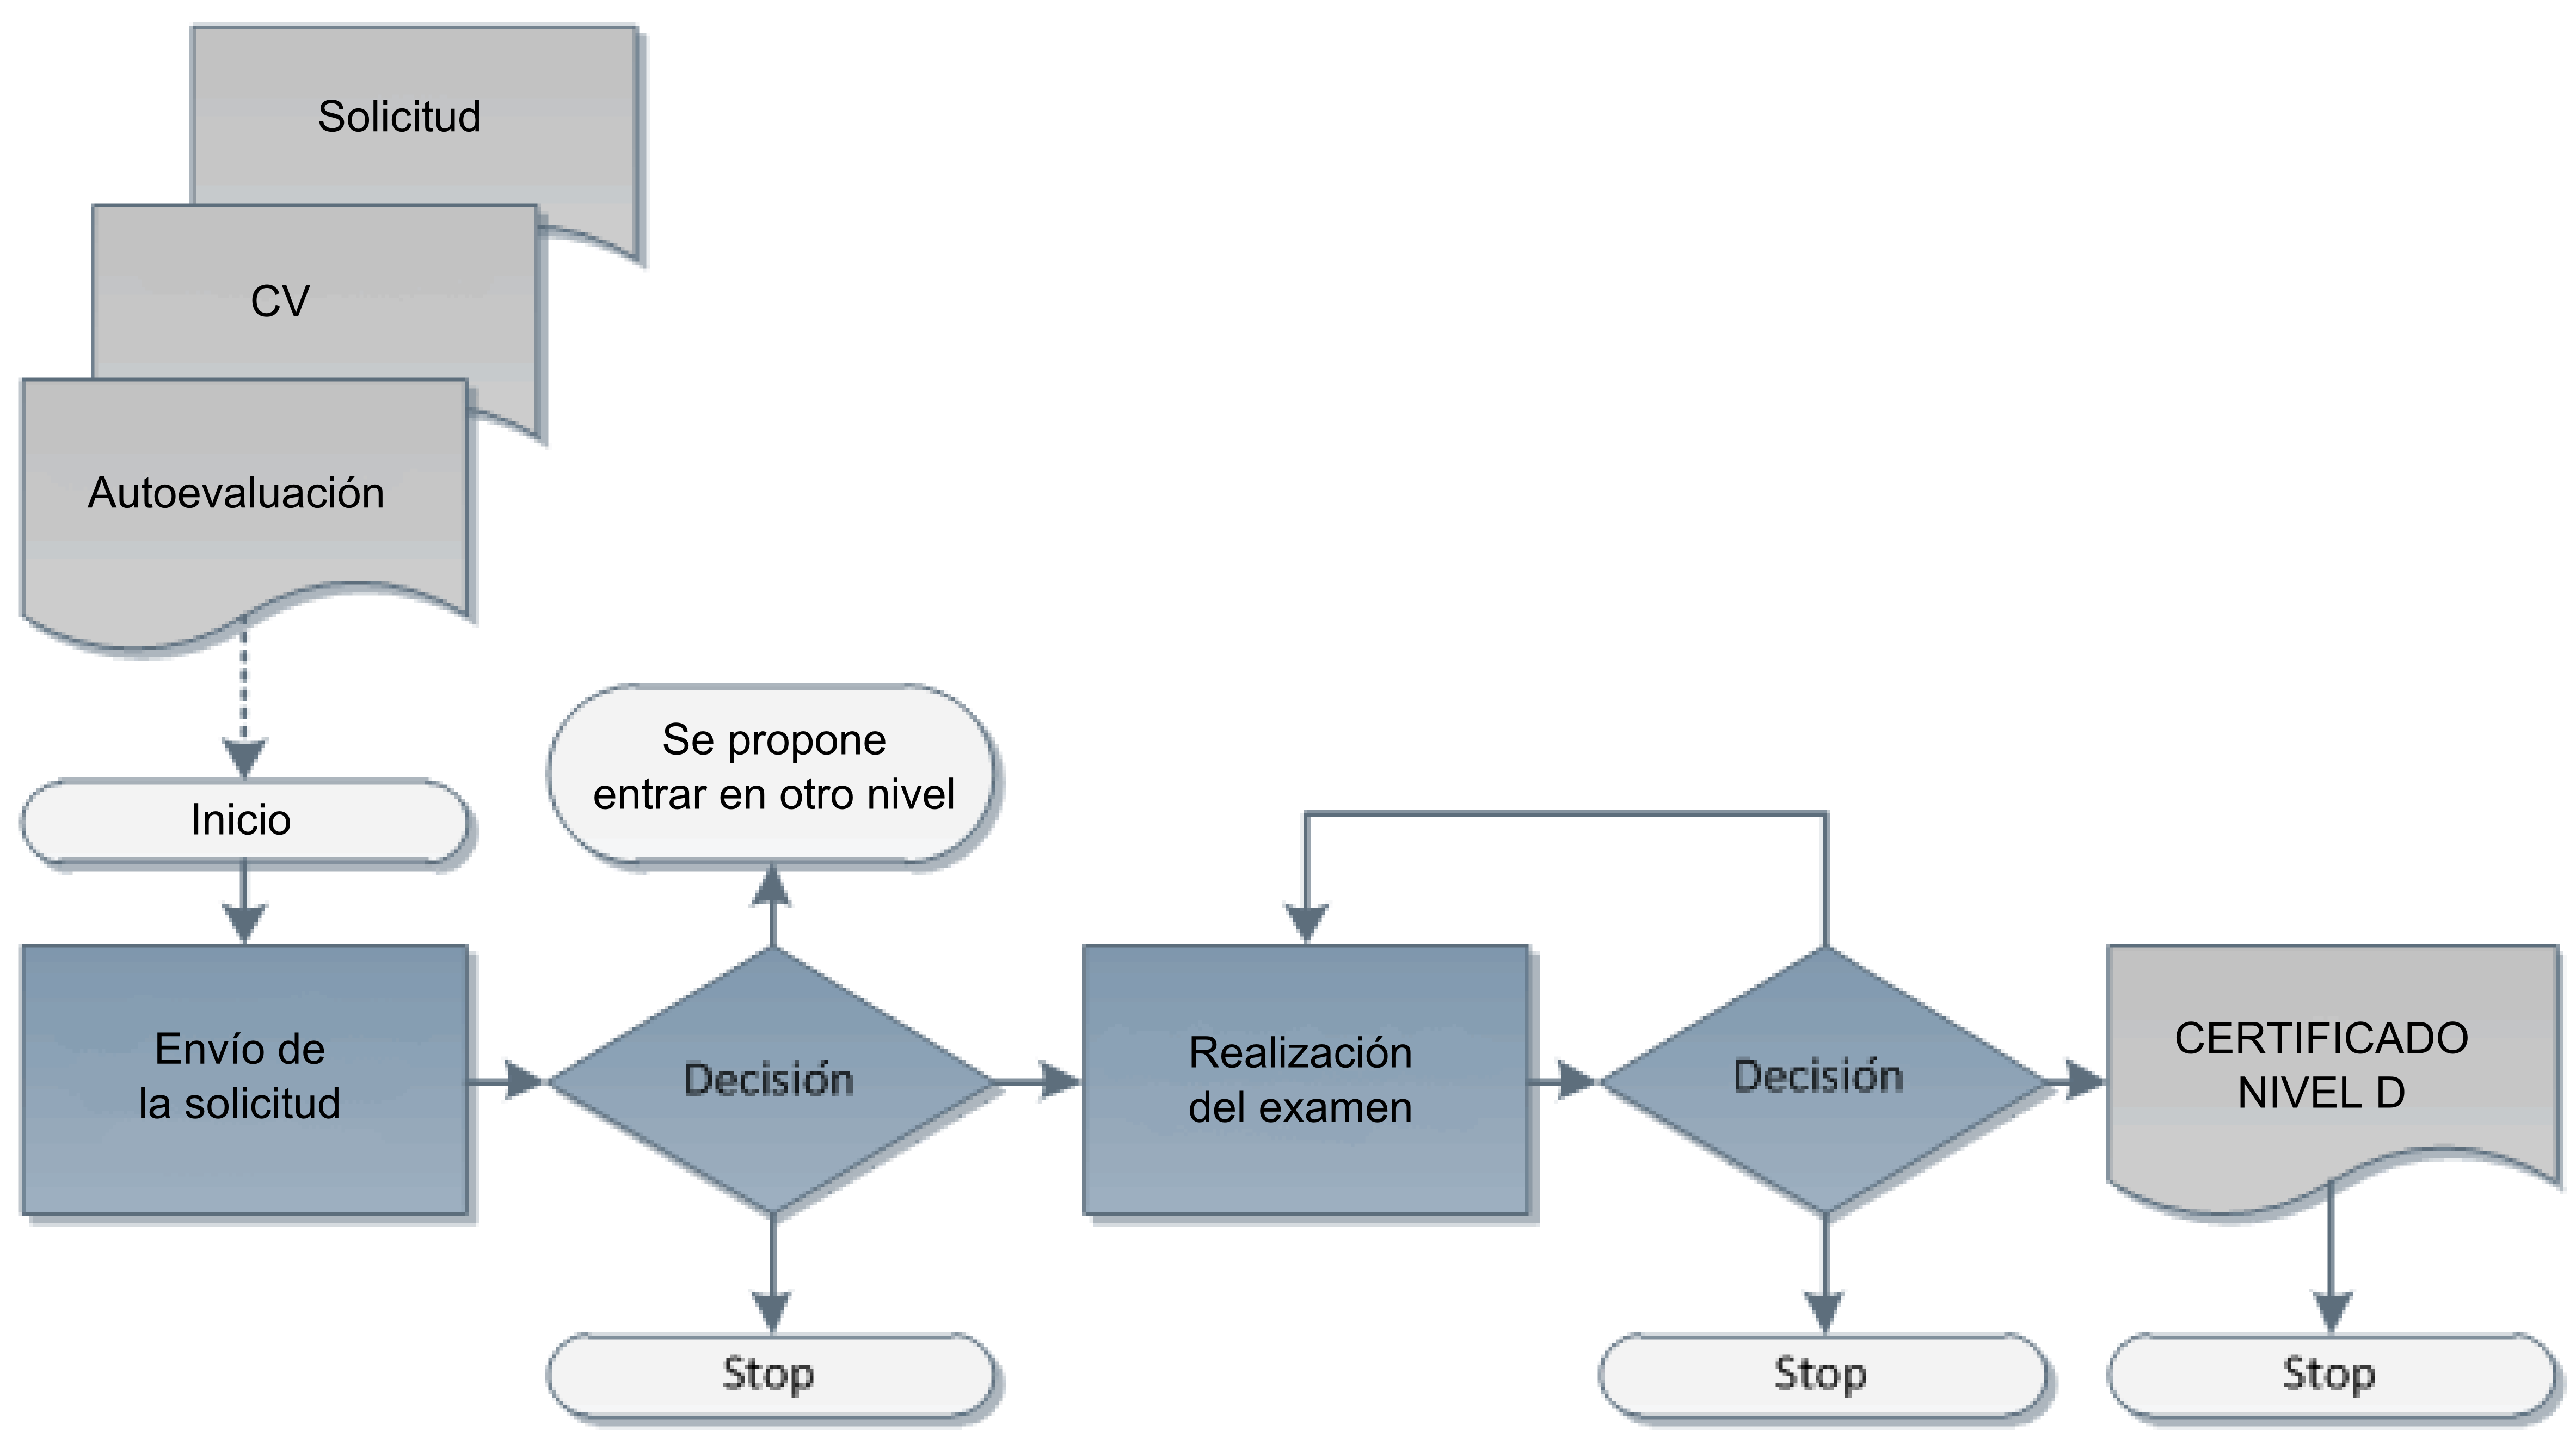
\includegraphics[height=4.5cm]{figuras/procesod.png}
			
			Diagrama de flujo del proceso de certificación.
		\end{center}
		
	\end{enumerate}
	
\end{frame}
